\documentclass[a4paper]{report}

%====================== PACKAGES ======================

\usepackage[french]{babel}
\usepackage[utf8]{inputenc}
\usepackage{graphicx} % Pour les images
\usepackage{float} % Pour gérer les positionnement d'images
\usepackage{amsmath} % Pour des équations plus jolies
\usepackage{url}
\usepackage[hidelinks]{hyperref} % Pour les liens internes et externes
\usepackage{array} % Pour la mise en page des tableaux
\usepackage{tabularx}
\usepackage{setspace} % Espacement entre les lignes
\usepackage{abstract} % Modifier la mise en page de l'abstract
\usepackage[T1]{fontenc}
\usepackage[top=3cm, bottom=4cm, left=3.5cm, right=3.5cm]{geometry} % Mise en page (marges) du document
\usepackage{subfig} % Pour les galeries d'images
\usepackage{titlesec} % Pour changer le style des titres
\usepackage[squaren,cdot]{SIunits} % Pour les unités
\usepackage[backend=biber,
			style=numeric,
			url=true,
			doi=false,
			isbn=false,
			backref=false]{biblatex} % Pour la bibliographie
\usepackage{enumitem}
\usepackage{wasysym}
\usepackage{eurosym} % Pour le symbole euro
\usepackage{textcomp}
\usepackage[toc,nonumberlist,nopostdot]{glossaries} % Pour faire un glossaire
\usepackage{lmodern}
\usepackage{csquotes} % Pour les guillemets
\usepackage{fontspec}
\setmainfont{Times} % Police
\usepackage{color} % Pour définir des couleurs personnalisées
\usepackage{listings} % Pour insérer du code
\definecolor{bluekeywords}{rgb}{0.13,0.13,1}
\definecolor{greencomments}{rgb}{0,0.5,0}
\definecolor{redstrings}{rgb}{0.9,0,0}
\lstset{language=[Sharp]C, % DEFINIR LE LANGAGE ICI
	showspaces=false,
	showtabs=false,
	breaklines=true,
	showstringspaces=false,
	breakatwhitespace=true,
	escapeinside={(*@}{@*)},
	commentstyle=\color{greencomments},
	keywordstyle=\color{bluekeywords}\bfseries,
	stringstyle=\color{redstrings},
	tabsize=4,
	basicstyle=\ttfamily
}
\lstset{literate= % Pour que listings gère l'UTF-8
	{á}{{\'a}}1 {é}{{\'e}}1 {í}{{\'i}}1 {ó}{{\'o}}1 {ú}{{\'u}}1
	{Á}{{\'A}}1 {É}{{\'E}}1 {Í}{{\'I}}1 {Ó}{{\'O}}1 {Ú}{{\'U}}1
	{à}{{\`a}}1 {è}{{\`e}}1 {ì}{{\`i}}1 {ò}{{\`o}}1 {ù}{{\`u}}1
	{À}{{\`A}}1 {È}{{\'E}}1 {Ì}{{\`I}}1 {Ò}{{\`O}}1 {Ù}{{\`U}}1
	{ä}{{\"a}}1 {ë}{{\"e}}1 {ï}{{\"i}}1 {ö}{{\"o}}1 {ü}{{\"u}}1
	{Ä}{{\"A}}1 {Ë}{{\"E}}1 {Ï}{{\"I}}1 {Ö}{{\"O}}1 {Ü}{{\"U}}1
	{â}{{\^a}}1 {ê}{{\^e}}1 {î}{{\^i}}1 {ô}{{\^o}}1 {û}{{\^u}}1
	{Â}{{\^A}}1 {Ê}{{\^E}}1 {Î}{{\^I}}1 {Ô}{{\^O}}1 {Û}{{\^U}}1
	{œ}{{\oe}}1 {Œ}{{\OE}}1 {æ}{{\ae}}1 {Æ}{{\AE}}1 {ß}{{\ss}}1
	{ű}{{\H{u}}}1 {Ű}{{\H{U}}}1 {ő}{{\H{o}}}1 {Ő}{{\H{O}}}1
	{ç}{{\c c}}1 {Ç}{{\c C}}1 {ø}{{\o}}1 {å}{{\r a}}1 {Å}{{\r A}}1
	{€}{{\euro}}1 {£}{{\pounds}}1 {«}{{\guillemotleft}}1
	{»}{{\guillemotright}}1 {ñ}{{\~n}}1 {Ñ}{{\~N}}1 {¿}{{?`}}1
}
\usepackage{comment} % Pour compiler sans les images
%\excludecomment{figure} % Décommenter pour compiler sans les images
%\let\endfigure\relax

%====================== INFORMATION ET REGLES ======================

\hypersetup{                            % Information sur le document
pdfauthor = {Pierre \textsc{Biret} et Victor \textsc{Fauth}},          % Auteurs
pdftitle = {Rapport de projet long - Conception de logiciel de simulation de circuit électrique},           % Titre du document
pdfstartview={FitH}}					 % Ajuste la page à la largueur de l'écran

\graphicspath{{Images/}}

\titleformat{\chapter}{\Huge}{\Roman{chapter}.}{20pt}{\Huge\normalfont}

\makeglossaries


%======================== DEBUT DU DOCUMENT ========================

\begin{document}

\begin{titlepage}
\begin{center}

% Upper part of the page. The '~' is needed because only works if a paragraph has started.

\includegraphics[width=0.7\textwidth]{logoCS}~\\[1cm]

\vspace{0.5cm}

{\LARGE 2\ieme{} année du cursus ingénieur Supélec - Projet long\\[0.4cm] }

{\Huge \bfseries Conception d'un logiciel de simulation de circuit électrique \\[0.4cm] }

\vspace{1.5cm}

\huge Pierre \textsc{Biret} et Victor \textsc{Fauth}, promotion 2019 \\[2cm]

\LARGE Année 2017-2018 \\[2cm]

\textit{Professeur encadrant :} Amir \textsc{Arzandé}


\end{center}
\end{titlepage} % Page de garde

\tableofcontents
\thispagestyle{empty}
\setcounter{page}{0}

\newpage

% !TeX root = ./rapport.tex
\chapter*{Introduction}
\addcontentsline{toc}{chapter}{Introduction}

\paragraph{}Dans le cadre de notre projet long de la deuxième année du cursus ingénieur à Supélec, nous devons développer un logiciel de simulation de circuit électrique. Il s'agit d'un logiciel qui permet à l'utilisateur de créer graphiquement un circuit électrique (à l'aide de composants génériques ou personnalisés) puis de simuler son fonctionnement dans différentes conditions. Un logiciel commercial de ce type parmi les plus connus est LTspice.

\paragraph{}Ce projet ayant déjà été proposé l'an dernier, il a été décidé que nous commencerions à partir de zéro afin de bien maîtriser chaque étape de la conception du logiciel. Cependant, nous conservons le langage de programmation précédemment utilisé. Le logiciel sera donc codé en C\#. Il s'agit d'un langage orienté objet, très inspiré du C++, mais développé par Microsoft dans le cadre de la plateforme .NET et présentant de nombreuses différences. Pour gérer le front-end, nous utiliserons WPF (\textit{Windows Presentation Foundation}).

\paragraph{}D'un point de vue organisationnel, le projet se déroulera en plusieurs phases : tout d'abord une phase de montée en compétences en codant un petit jeu, puis l'implémentation d'une interface graphique basique pour le programme. Cela nous permettra ensuite d'ajouter la simulation du circuit. S'il nous reste du temps, nous pourrons ajouter des fonctionnalités au programme pour le rendre plus agréable, intuitif et rapide à utiliser.

\newpage

%====================== INCLUSION DES PARTIES ======================

\chapter{Montée en compétences : programmation d'un programme simple}

\paragraph{}Afin d'apprendre à coder en C\# avec WPF, nous avons décidé de commencer par un projet bien plus modeste : le développement d'un jeu de Memory. Il s'agit d'apprendre à coder en C\# avec WPF (et donc à utiliser XAML, comme expliqué au prochain paragraphe), mais aussi de se familiariser avec l'IDE utilisé. Nous avons choisi pour cela Microsoft Visual Studio : le langage C\# a été créé pour être utilisé avec cet IDE, il permet de générer le code XAML à partir d'une interface graphique, possède des outils de déboguage très puissants et une licence est fournie aux élèves de Supélec. Comme gestionnaire de versions, nous utilisons Git.

\begin{figure}[h]
	\begin{minipage}[t]{0.5\textwidth}
		\centering
		
\includegraphics[height=1cm, width=\textwidth, keepaspectratio=true]{logoVS.png}		
	\end{minipage}
	\begin{minipage}[t]{0.5\textwidth}
		\centering
		
\includegraphics[height=1cm, width=\textwidth, keepaspectratio=true]{logoGit.png}		
	\end{minipage}
	\caption{Les logos de Visual Studio 2017 (gauche) et de Git (droite).}
	\label{fig:logos}
\end{figure}


\section{La dualité C\#/XAML}

\paragraph{}Lorsqu'un programme graphique est créé en utilisant WPF, deux langages sont utilisés. Les éléments graphiques (fenêtre, boutons, images, etc...) sont codés en XAML. Il s'agit d'un langage descriptif dérivé du XML. Il nous permet de décrire les attributs de chaque élément : par exemple, la fenêtre a un nom (utilisé pour l'appeler dans le code), un titre, une taille, une position, etc... Elle possède aussi des \enquote{children} : par exemple, un bouton. Ce bouton possède des attributs similaires, mais aussi certains attributs spécifiques, tels l'animation à effectuer lors de l'activation. Si une fonction à lancer au clic (ou lors de n'importe quel événement ayant lieu sur l'élément) peut être définie pour la fenêtre, cet attribut est obligatoire pour un bouton.

\paragraph{}Le XAML est un langage qui permet ainsi de définir rapidement une interface utilisateur, sans qu'il soit nécessaire de taper trop de code. Tous les éléments sont aussi personnalisables si nécessaire, bien que cela soit assez complexe. 

\paragraph{}Le code lui-même est écrit en C\#. Il gère toute la logique et l'interactivité du programme. Si une interactivité est nécessaire, par exemple pour changer le titre de la fenêtre au clic, il est possible de modifier tous les éléments depuis le code, d'en créer ou d'en supprimer.

\begin{figure}[H]
	\centering
	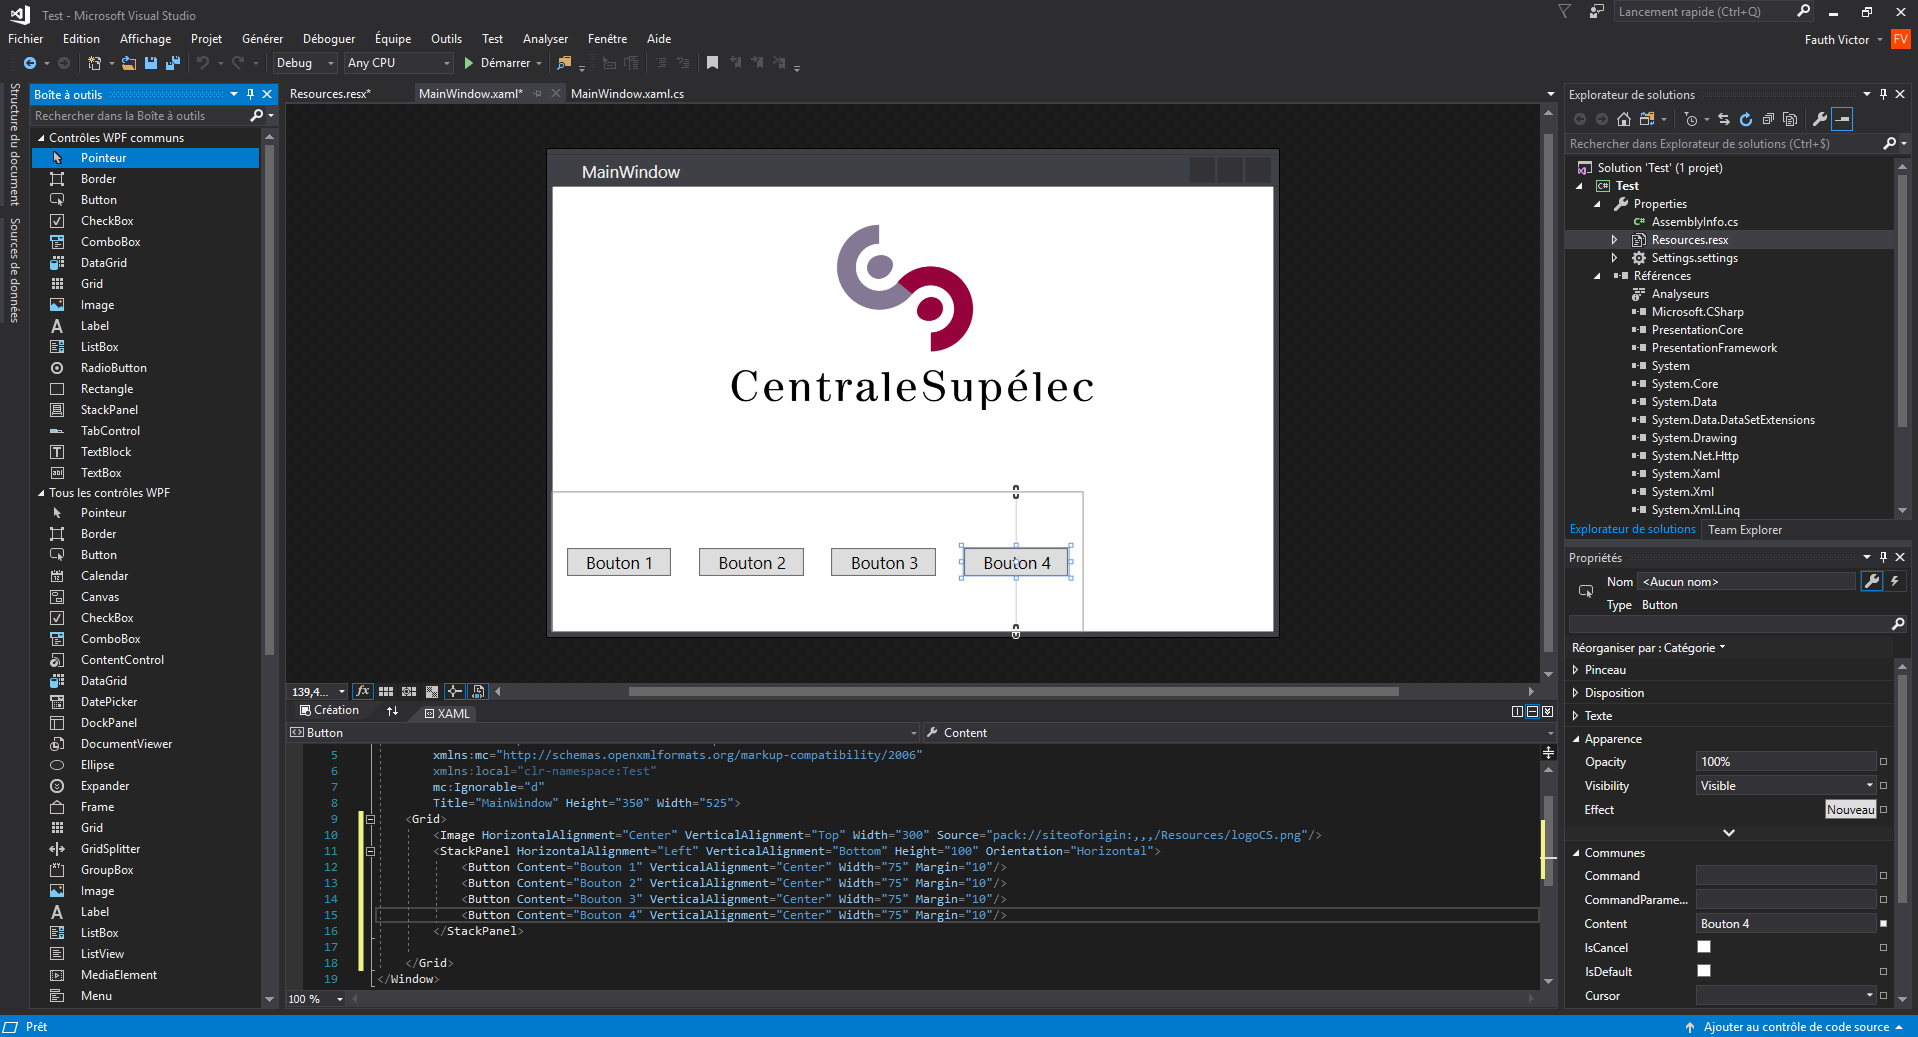
\includegraphics[width=1\textwidth]{editorXAML.png}
	\caption{L'éditeur graphique de XAML. Ici, une fenêtre avec une image et une ligne de boutons a été créée grâce à l'outil graphique, le code XAML correspondant est affiché dans la fenêtre inférieure. La fenêtre de droite permet de modifier les propriétés de l'élément sélectionné.}
	\label{fig:editorXAML}
\end{figure}


\section{Règles du jeu}

\paragraph{}Il s'agit d'un jeu très simple dans lequel un certain nombre de cartes sont posées, face cachée. Ces cartes vont par paire : chaque motif est représenté sur deux cartes. Les cartes sont posées au hasard, puis le joueur retourne deux cartes. Si elles sont identiques, la paire est retirée du jeu. Sinon, elles sont retournées face cachée, au même endroit (après un temps, ici deux secondes, permettant au joueur de mémoriser les cartes). Le jeu s'arrête lorsque toutes les paires ont été trouvées, le but étant de minimiser le nombre d'essais.


\section{Implémentation}

\subsection{Le modèle MVC}

\paragraph{}Pour coder le jeu, nous avons décidé d'utiliser l'architecture MVC (Modèle-Vue-Contrôleur). Le principe est de séparer le code en trois composantes distinctes : le modèle contient les données du programme, le contrôleur gère la logique et la vue interagit avec l'utilisateur.

\begin{figure}[H]
	\centering
	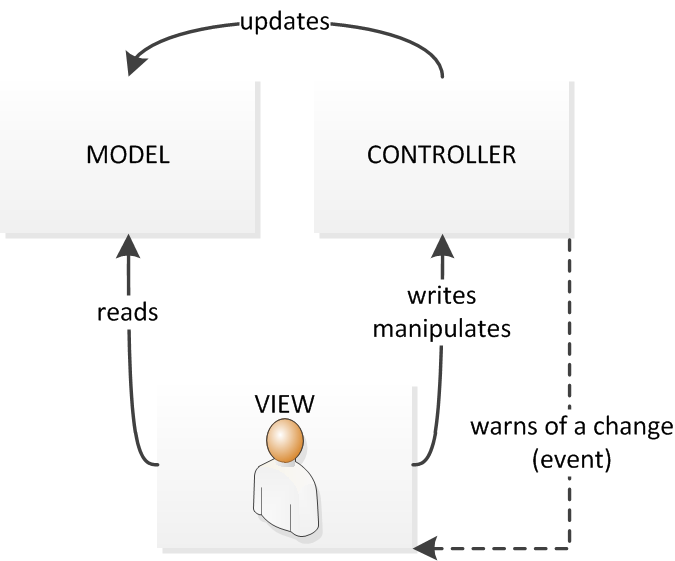
\includegraphics[width=1\textwidth]{modeleMVC.png}
	\caption{Les interactions de l'architecture MVC. Image tirée de Wikipédia.}
	\label{fig:MVC}
\end{figure}

\paragraph{\textbf{Remarque}} La structure de chaque classe est donnée en \autoref{sec:memory_annexe}.
\subsubsection{Le modèle}

\paragraph{}Le modèle contient l'état du jeu a un moment donné. Pour cela, nous définissons deux classes : la classe \lstinline|Card| et la classe \lstinline|Board|. \lstinline|Card| représente une carte et définit son état (trouvée et/ou affichée) ainsi que la pair dont fait partie la carte, tandis que \lstinline|Board| représente tout le plateau de jeu et contient notamment toutes les cartes, ainsi que le compteur de tours pour la partie en cours. Il possède une méthode pour incrémenter ce compteur, appelée à chaque fois que le joueur a désigné deux cartes, et deux méthodes utilisées lors de l'initialisation du plateau de jeu.


\subsection{Le contrôleur}

\paragraph{}Le contrôleur a la responsabilité de toute la logique du jeu. Il possède peu d'attributs, le stockage des données étant du ressort du modèle : deux attributs servent juste à référencer la vue et le plateau de jeu, le troisième enregistre quelle carte a été choisie par le joueur en attendant qu'il en choisisse une seconde. 

\paragraph{}Il y a cependant bien plus de méthodes, qui sont appelées lorsque le joueur agit. La méthode \lstinline|CardChosen| est appelée lorsque le joueur choisit une carte. S'il en a déjà choisi une juste avant, cette méthode vérifie si les deux cartes forment une paire avec \lstinline|CheckPair|, puis agit en conséquence. La méthode \lstinline|NextTurn| est alors appelée, et prépare le tour suivant, notamment en cachant à nouveau les cartes choisies précédemment (si elles ne constituaient pas une paire). C'est aussi elle qui va gérer la fin du jeu avec les méthodes \lstinline|IsFinished| (qui renvoie une booléen indiquant si toutes les paires ont été trouvées ou non ) et \lstinline|Exit| qui demande à la vue d'afficher la fenêtre de fin de partie.

\subsection{La vue}

\subsubsection{L'interface graphique statique en XAML}

\paragraph{}Le jeu gère n'importe quel nombre (pair) de cartes, nous n'avons donc pas défini l'interface graphique de manière statique en XAML : la classe \lstinline|Display| se charge de créer la totalité de l'affichage et de charger les images présentes dans le dossier pour les afficher en fonction du nombre de cartes souhaité. Le code XAML est donc presque vide, seule un élément \lstinline|Grid| est défini. Celui-ci s'étend sur l'intégralité de la surface de la fenêtre et permet juste de positionner facilement les cartes.


\subsubsection{L'interactivité en C\#}

\paragraph{}La classe \lstinline|Display| contient donc toutes les méthodes pour charger les images, créer les cartes à partir de ces images et des données du modèle, afficher et rafraîchir le plateau de jeu, et afficher la fenêtre des scores en fin de partie. Il s'agit de la classe la plus complexe à coder : pas à cause de sa logique, mais parce que cela a nécessite de bien comprendre le fonctionnement de WPF. Si le contrôleur et le modèle furent assez simple à coder, c'est parce qu'il s'agissait de programmation \enquote{générique}, à laquelle nous sommes déjà habitués, et le C\# n'est pas un langage extrêmement complexe à prendre en main si nous sommes déjà habitués au C++ ou au Java. Cependant, le WPF est extrêmement particulier, et, bien qu'il soit extrêmement puissant, de nombreux concepts sont difficiles à prendre en main et nécessitent de se plonger dans la documentation. Cela fut très instructif, nécessaire pour la suite du projet, et surtout formateur. 


\begin{figure}[H]
	\centering
	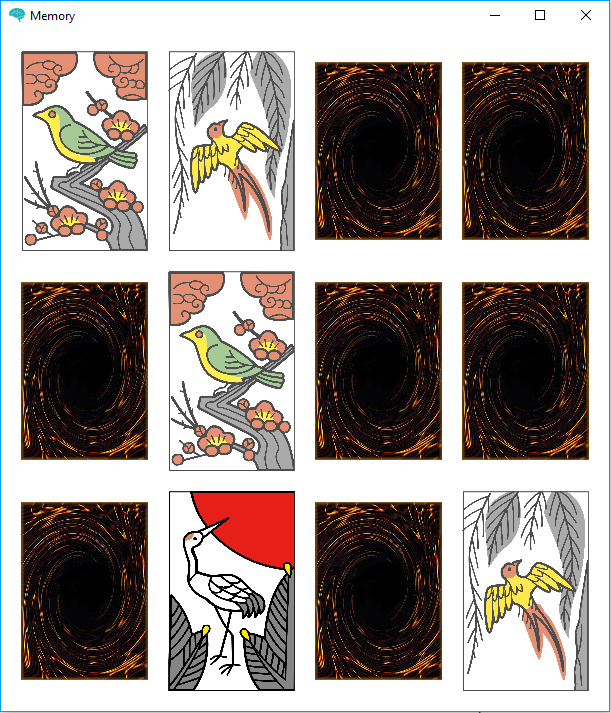
\includegraphics[width=1\textwidth]{memory.png}
	\caption{Une partie avec 16 cartes. Deux paires ont été trouvées, et une carte a été sélectionnée.}
	\label{fig:memory}
\end{figure}

\newpage
\subsection{Annexe}
\label{sec:memory_annexe}

\lstinputlisting[caption=La structure de la classe \lstinline|Card| du modèle.]{Sources/Memory/Model/Card.cs}
\newpage
\lstinputlisting[caption=La structure de la classe \lstinline|Board| du modèle.]{Sources/Memory/Model/Board.cs}
\newpage
\lstinputlisting[caption=La structure de la classe \lstinline|Game| du contrôleur.]{Sources/Memory/Controller/Game.cs}
\newpage
\lstinputlisting[caption=La structure de la classe \lstinline|Display| de la vue.]{Sources/Memory/View/Display.cs}


%% !TeX root = ./rapport.tex
\chapter{Cahier des charges et organisation}

\paragraph{}Le but est de développer un logiciel permettant la saisie de circuits électriques ainsi que la simulation de leur comportement. Il n'est pas attendu un logiciel de qualité professionnelle devant être effectivement utilisé : nous nous limitons donc à des fonctionnalités d'édition basiques (création, sauvegarde et chargement de circuits de taille limitée), avec une liste de composants disponibles réduite (source de tension alternative ou continue, source de courant, résistance, inductance, condensateur, fil et terre) et un fonctionnement de la simulation limité à des cas simples. Il n'y a pas de liste spécifique de capacités à remplir, mais nous avons une année pour faire du mieux possible.

\paragraph{}Le professeur encadrant nous ayant laissé une grande latitude organisationnelle, nous avons décidé d'organiser ce projet en deux grandes phases : tout d'abord, nous allons nous occuper du front-end, avec les capacités d'édition du circuit, puis du back-end, pour permettre les simulations. Cette première partie nous a pris 2 séquences scolaires sur 4 (le Memory en avait déjà occupé une), de début décembre à début mars. La dernière séquence sera donc allouée à la simulation, avec une approche itérative : l'algorithme sera complété au fur et à mesure afin de permettre de simuler des cas plus complexes avec des résultats plus précis.

%\chapter{Implémentation}


%\newpage
%\chapter*{Conclusion}
\addcontentsline{toc}{chapter}{Conclusion}




\newglossaryentry{IDE}
{
	name=IDE,
	description={L'environnement de développement intégré (IDE en anglais) est un logiciel permettant à la fois d'éditer du code et de le compiler. Il comprend généralement des outils simplifiant le développement, tels une coloration syntaxique, une auto-complétion du code ou un débogueur.}
}

\newglossaryentry{frontend}
{
	name=Front-end,
	description={Le front-end représente la partie d'un logiciel (et donc le code associé) qui interagit avec l'utilisateur. Il s'agit donc de l'interface entre le back-end et l'utilisateur.}
}

\newglossaryentry{backend}
{
	name=Back-end,
	description={Le back-end représente la partie d'un logiciel (et donc le code associé) qui gère la logique et le fonctionnement interne d'un logiciel.}
}



\glsaddall % Pour afficher toutes les entrées du glossaire
\printglossaries


\end{document}